\begin{figure*}[t]
    \centering
    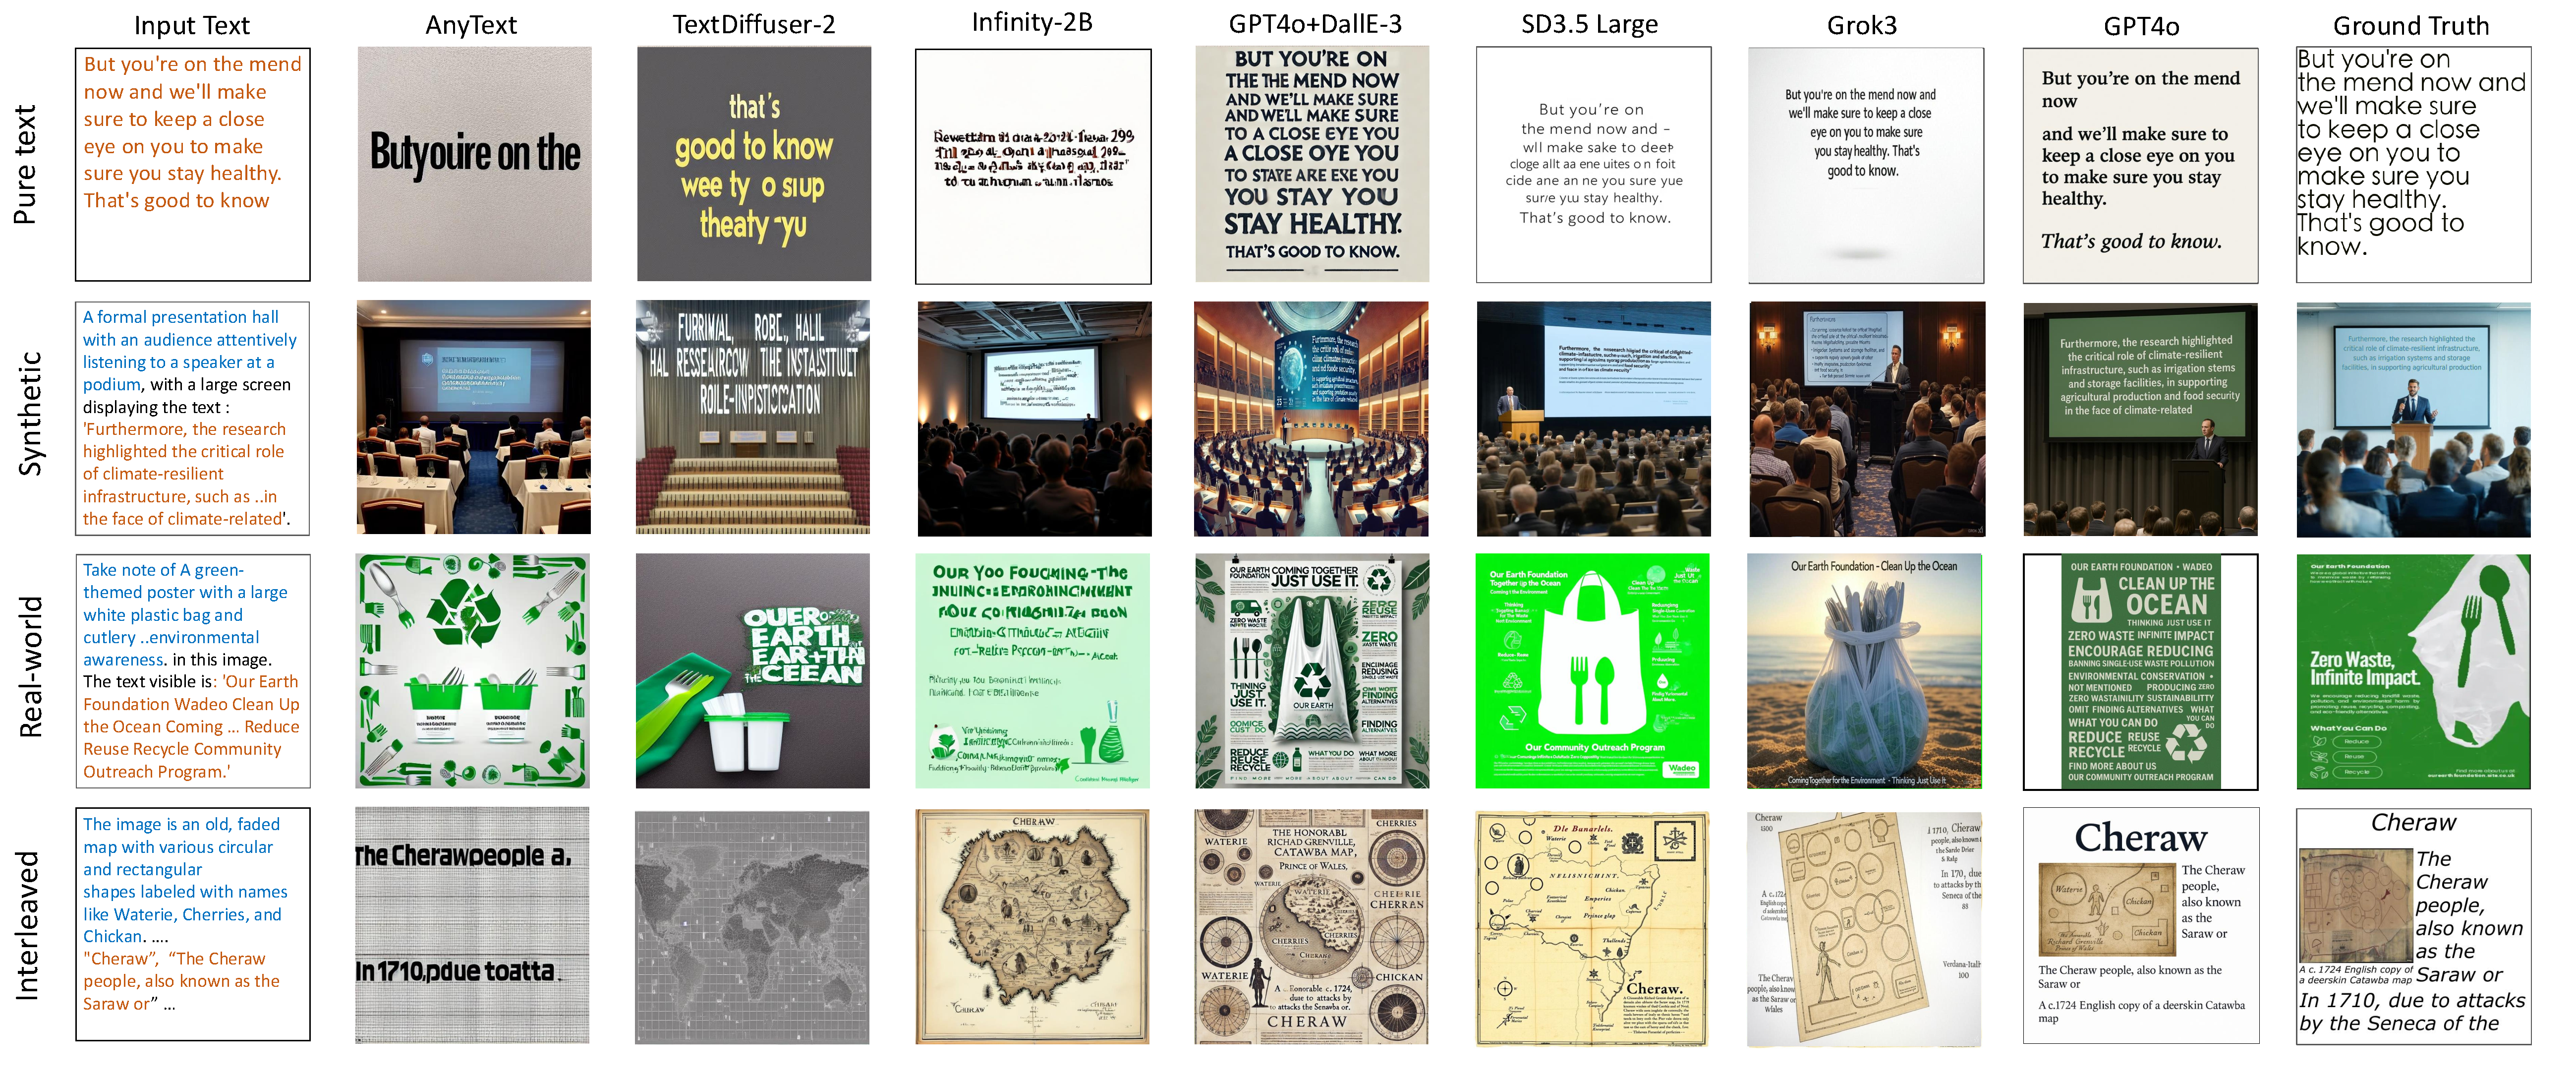
\includegraphics[width=\linewidth]{Appendix/images/text_only_data_v2.pdf}
    \vspace{-1em}
    \caption{
    \textbf{Long text image generation remain challenge for existing model.}
    Existing public methods, such as AnyText~\cite{anytext} and Text Diffuser2~\cite{textdiffuser2}, are capable of rendering short text but struggle with longer sequences. 
    In contrast, GPT4o~\cite{gpt4o} and SD3.5 Large~\cite{sd3} show superior performance, though they still produce inaccuracies such as duplicated words or missing letters when handling extended text.
    For interleaved documents, all methods perform poorly due to their lack of layout planning capabilities.
    The yellow highlights text, while the blue indicates scene descriptions.
    }
    \label{fig:t2i_evaluation}
\end{figure*}